so solution

\section{Arithmetic logic unit}
	\label{s:ALU}
	
	The arithmetic logic unit, ALU, is the core of the processors computing and is what preform the integer arithmetic and logical operations. 

An ALU implemented were able to do addition and subtraction as well as shift left and logical ``and'' and ``or''. An early RTL sketch of the planned implementation is shown in figure \ref{fig:alu}.
	
	\begin{figure} [H]
		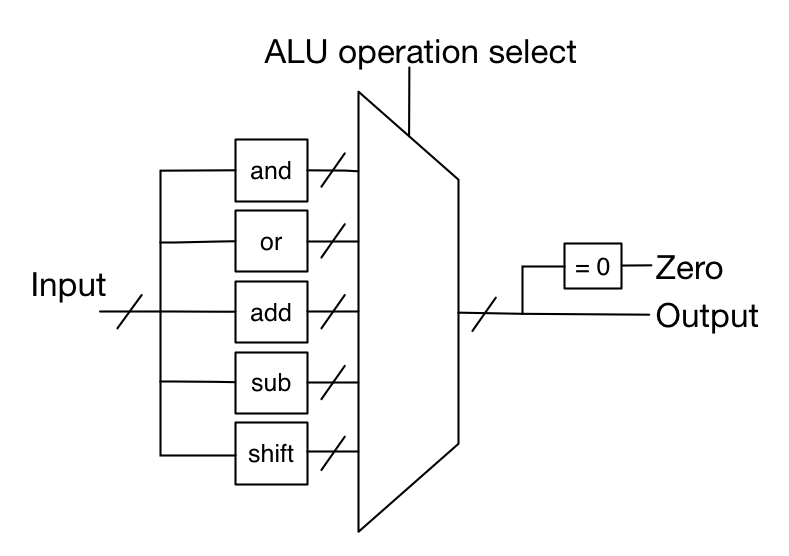
\includegraphics[scale=1]{RTL/ALU.png}
		\caption{RTL scotch of the ALU.}
			\label{fig:alu}
	\end{figure}
	
	The $input$ contains a vector of which the operations will be preformed on. The outgoing resulting vector will be decided by the $ALU operation select$ via a multiplexer. Then the output will then hold the result chosen by the multiplexer. If all bits in the outgoing vector are zero the $Zero$-flag will be set high.